Обновлением виртуальной машины, или неудачная попытка настройки или просто какая-то ошибка при её запуске, может привести к потери ценных данных, а на переустановку системы и настройку программ может уйти очень много времени. Именно для таких случаев и предназначены снимки в VirtualBox. Они нужны для сохранения прогресса на случай непредвиденной поломки машины и отката до ранее стабильного состояния. Поэтому перед и после обновления или установки чего-то важного, стоит делать снимки.

Для создания снимка своей виртуальной машины нужно нажавть на кнопку с изображением фотоаппарата с плюсом.

Снимок можно удалить, восстановить и посмотреть на его свойства на момент его создания.

\begin{figure}[h]
		\centering
		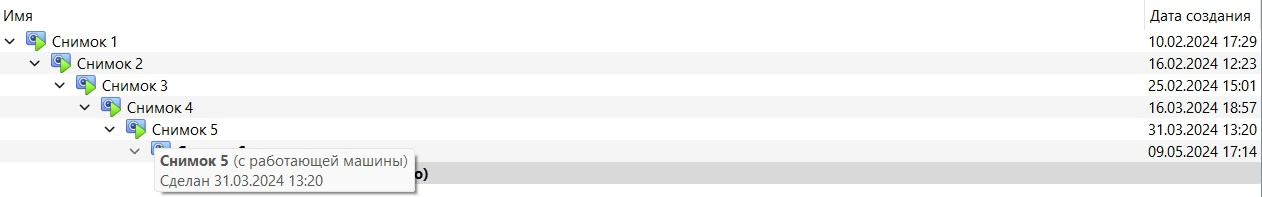
\includegraphics[width=1\linewidth]{VM/s2.jpg}
\caption{Дерево снимков.}
\label{ris:image}
\end{figure}

При создании можно оставить название по умолчанию и не вводить никакого описания, но если таких снимков в будущем накопится много, можно будет запутаться. 

\begin{figure}[h]
		\centering
		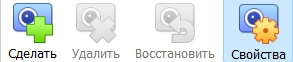
\includegraphics[width=0.8\linewidth]{VM/s3.jpg}
\caption{Действия со снимками.}
\label{ris:image}
\end{figure}

Для восстановления состояния виртуальной машины нужно выбрать нужный нам снимок, и нажать «Восстановить снимок».
 
VirtualBox предложит дополнительно создать снимок текущего состояния системы. Нужно поставить галочку и нажать кнопку «Восстановить». чтобы, иметь возможность вернуться к  текущему состоянию, если была совершена ошибка или снимок оказался не тот, что нужен.
 
\begin{figure}[h]
		\centering
		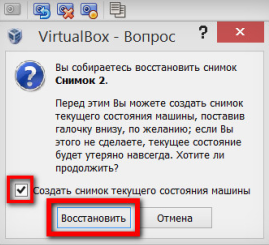
\includegraphics[width=0.4\linewidth]{VM/s4.png}
\caption{Восстановление снимка.}
\label{ris:image}
\end{figure}

Далее можно дать снимку текущего состояния имя и описание и нажать кнопку «ОК».

После VirtualBox вернёт состояние системы к моменту создания выбранного снимка.

